\pdfoutput=1

\documentclass[11pt]{article}

\usepackage[final]{final}
\usepackage{times}
\usepackage{amsfonts}
\usepackage{latexsym}
\usepackage[T1]{fontenc}
\usepackage[utf8]{inputenc}
\usepackage{microtype}
% \usepackage{inconsolata}
\usepackage{graphicx}
\usepackage{float}
\title{Efficient Image Compression}

\author{James Camacho \\
  MIT / AI \\
  \texttt{jamesc03@mit.edu} \\\And
  Linda He \\
  Harvard / Applied Mathematics \\
  \texttt{lindahe@college.harvard.edu} \\}

\begin{document}
\maketitle
\begin{abstract}
  With high-dimensional spaces such as images or video, perfect communication becomes prohibitively expensive. A lossy compressed version is cheaper to transmit and good enough for most purposes. Traditional algorithms such as JPEG use a Fourier transform to pick out the most important features for transmission. In this paper, we explore using auto- and raster-encoders to automatically and efficiently compress images instead. We find they significantly outperform JPEG on the MNIST dataset, and discuss potential future improvements to their speed and cost via reinforcement learning.
\end{abstract}


\section{Introduction}

Over 75\% of internet traffic comes in the form of video \citep{cisco-2018-traffic}, and YouTube alone runs a \$30bn business from their distribution \citep{alphabet-2024-earnings}. At these massive scales, every bit of transmission is important. In this paper, we explore more optimal compression, in part inspired from language models. As video is rather compute-intensive to train, we restrict ourselves to the MNIST image dataset.

Image and text have often been treated as separate domains, but there is much that can be applied between the two. Inspired by quantization and fractalization from image compression, Witten \textit{et al.} proposed several lossy text encoding schemes as far back as 1992 \citep{witten-etal-1992-lossy}. Recent advances in image generation such as denoising models \citep{ho-2020-denoising} have similarly found applications in text generation by interpreting language tokens as pixels \citep{kou-2024-cllms}. Going the other direction, the popular transformer architecture of language models have been applied to vision \citep{dosovitskiy-2021-vit}, and has seen state-of-the-art success in video production \citep{liu-2024-sora}.

This ``vision transformer'' architecture bears a striking resemblance to JPEG which is no coincidence. Generation is the inverse of compression, and more generally ``being able to compress well is closely related to acting intelligently'' \citep{hutter-2020}. Unfortunately, this enforces a tradeoff between the algorithm's speed and size. For example, an unintelligent compressor may store images verbatim, or a generator may simply sample from its training dataset. Smarter algorithms will do much better, but require more computation.

It would be interesting to explore this compute-compression tradeoff in more depth, but this paper will focus mostly on the tradeoff between quality and compression.

\section{Data}

We use the MNIST dataset with separate train and test sets. MNIST has $28\times 28$ greyscale images with values in the range $[0, 1]$, quantized to 8 bits. A sample image can be seen in Figure \ref{fig:recon}.

\section{Methods}
\subsection{JPEG}
We use JPEG as a baseline to compare against. The steps in JPEG compression are roughly:
\begin{enumerate}
    \item Colorspace Conversion: RGB images are converted to YCbCr format (a holdout from \th e olde days of black-and-white television). Our images are already in greyscale, i.e. solely the Y channel. If they had color, the Cb and Cr colors would be downsampled.
    \item Discrete Cosine Transform (DCT): The image is divided into $8\times8$ pixel blocks, and a DCT is applied to each block, converting the spatial image data into the frequency domain.
    \item Quantization: The low frequencies contain most of the important features of an image, so the higher frequencies are more aggressively quantized. The degree of quantization is controlled by a ``quality'' setting.
    \item Entropy Coding: The quantized DCT coefficients are then compressed using lossless entropy coding techniques like Huffman coding or arithmetic coding.
\end{enumerate}
The purpose of the DCT is to extract ``important'' features. Convolutional neural networks are known to automatically extract important features \citep{erhan-2009-features}, so our first experiment will be against them. The entropy coding looks very similar to how language models are trained, so our second experiment we will train a model in an LLM fashion.

\subsection{Auto-Encoders}

\begin{figure*}[p]
  \centering
  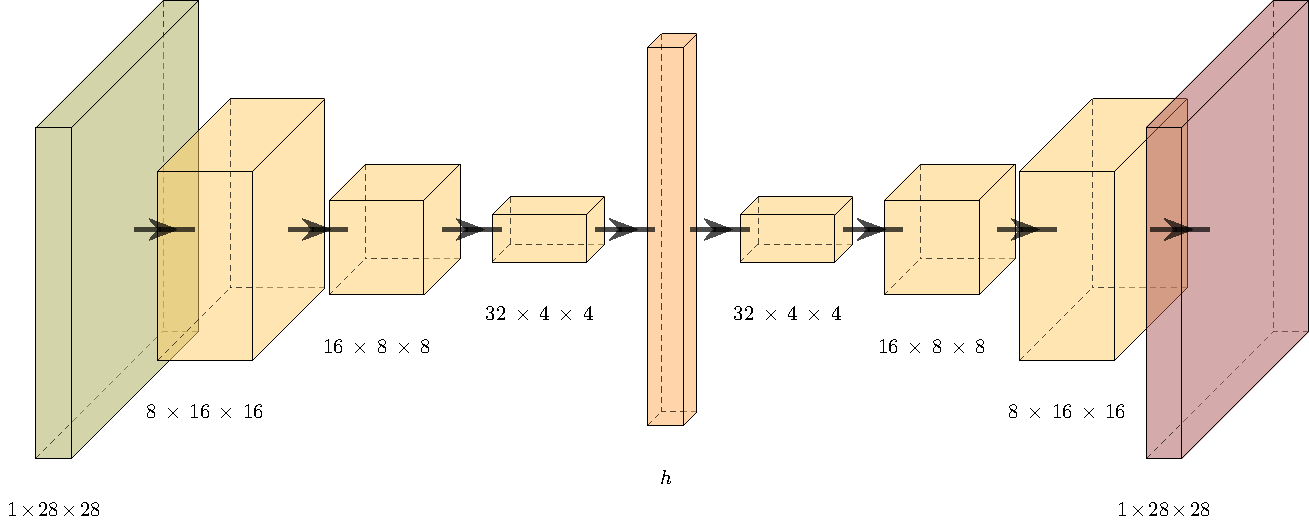
\includegraphics[width=1.5\columnwidth]{diagrams/auto.pdf}
  \caption{Auto-encoder network.}
  \label{fig:auto}
\end{figure*}

\begin{figure*}
  \centering
  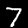
\includegraphics[width=0.2\columnwidth]{diagrams/reconstructions/original.png}
  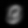
\includegraphics[width=0.2\columnwidth]{diagrams/reconstructions/0.png}
  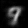
\includegraphics[width=0.2\columnwidth]{diagrams/reconstructions/1.png}
  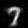
\includegraphics[width=0.2\columnwidth]{diagrams/reconstructions/2.png}
  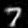
\includegraphics[width=0.2\columnwidth]{diagrams/reconstructions/4.png}
  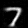
\includegraphics[width=0.2\columnwidth]{diagrams/reconstructions/8.png}
  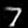
\includegraphics[width=0.2\columnwidth]{diagrams/reconstructions/16.png}
  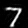
\includegraphics[width=0.2\columnwidth]{diagrams/reconstructions/32.png}
  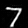
\includegraphics[width=0.2\columnwidth]{diagrams/reconstructions/64.png}
  \caption{Reconstructions of a sample image (left). To the right, $h=0, 1, 2, 4, 8, 16, 32, 64$.}
  \label{fig:recon}
\end{figure*}

Auto-encoders consist of an encoder and a decoder network trained together. Our encoder consists of three convolutional layers and a linear layer to control the latent dimension $h$, and the decoder has the reverse process (see Figure \ref{fig:auto}). By default, PyTorch stores floats using four bytes, so the encoding takes $4h$ bytes.

To train, we use the mean-squared error between the original and decoded images, running through two epochs of the MNIST training set with the Adam optimizer at $\gamma=10^{-3}$. We keep a separate dataset for testing. Sample reconstructions can be seen in Figure \ref{fig:recon}. As expected, the quality improves as the latent dimension increases, though the reconstructions remain blurry. This is an artifact of our loss function. Minimizing the squared error,
$$L_2 = \sum (x-\mathrm{correct})^2$$
is equivalent to maximizing the log-likelihood under a Gaussian prior for the error function:
$$L_2 = \log\prod e^{(x-\mathrm{correct})^2}.$$
The actual distribution of error is decidedly not Gaussian (Figure \ref{fig:hist}), so this biases the reconstruction towards a higher entropy than necessary. A common fix is to add a small adversarial loss \citep{makhzani-2016-adversarial}, but since our quality metric is the $L_2$ loss, we opt to keep the bias. We will use this bias to improve our raster-encoder.

\begin{figure}[H]
  \centering
  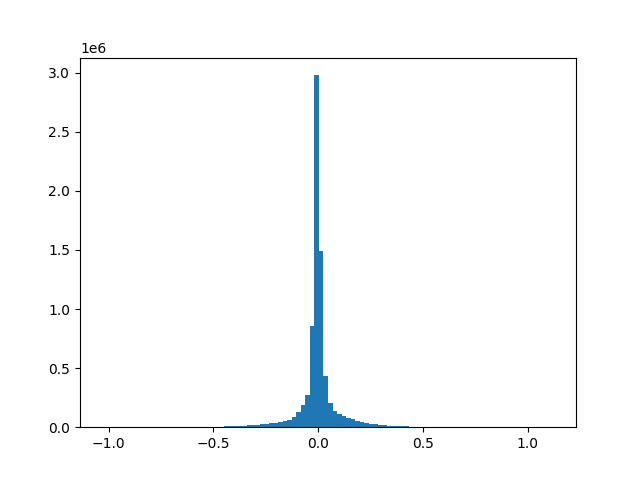
\includegraphics[width=\columnwidth]{diagrams/hist.png}
  \caption{Error histogram, 100 bins.}
  \label{fig:hist}
\end{figure}

\subsection{Raster-Encoders}

\begin{figure*}
  \centering
  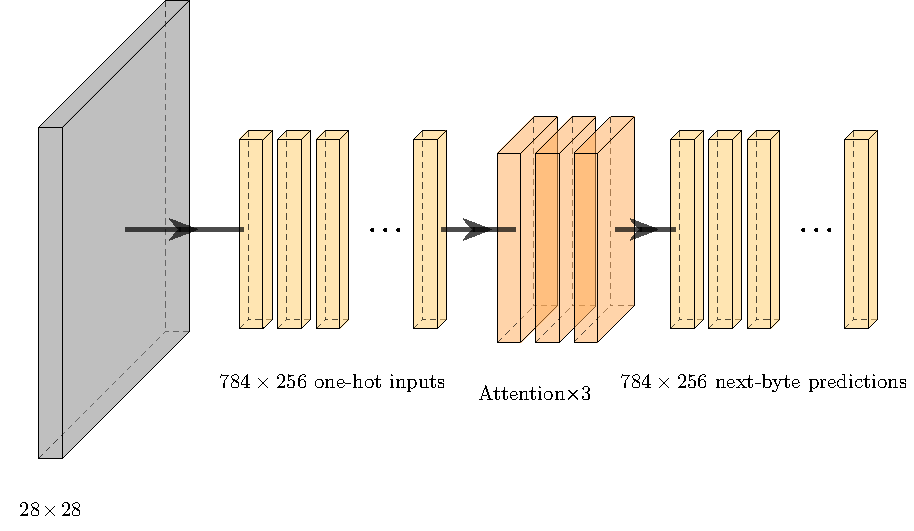
\includegraphics[width=1.5\columnwidth]{diagrams/raster.pdf}
  \caption{Raster-encoder network.}
  \label{fig:raster}
\end{figure*}

In \th e olde days, television was broadcast pixel by pixel, row by row, until an entire frame was drawn. This ``raster'' pattern flattens images into one-dimension, which we use to train models in a language-model style.

Originally we converted the grayscale images to RGB and pulled apart the individual bits, so a $28\times 28\times 8$ bit grayscale image became a sequence of $T=18816$ tokens. This is too large for attention, being over a gigabyte per head dimension ($4T^2\approx 1.4\mathrm{GB}$), so we used the state-space model Mamba \citep{gu-2023-mamba}. It uses a scan algorithm and takes $O(T)$ memory and $O(T\log T)$ time, as opposed to $O(T^2)$ for attention.

Unfortunately, we ran into software/hardware issues when scaling up, and didn't want to implement Mamba from scratch, so we switched to transformers. To reduce the sequence length, we kept our images grayscale and used bytes rather than bits for our tokens, giving a sequence of $784$ tokens with $256$ one-hot dimensions (Figure \ref{fig:raster}).

To compress, we can use arithmetic encoding on the output probabilities. Let $p(x)$ be the probability the next-byte prediction is $x$ and $q(x)$ the distribution of bytes encountered (i.e. in the training set). We want to minimize the compression length,
$$\mathbb{E}_q[-\log p] = \sum q\log p,$$
i.e. the traditional cross-entropy loss. Since the MNIST dataset is relatively small, the training data is unlikely to perfectly match the underlying image distribution. To fix this, we can inject extra entropy into $q$ while minimizing the expected error. We wish to minimize
$$L_2 = \mathbb{E}_q[(x-\mathrm{correct})^2] = \sum (x-\mathrm{correct})^2q(x)$$
for a fixed entropy
$$H(q) = -\sum q\log q.$$
Lagrange multipliers give
$$q\propto e^{-\beta(x-\mathrm{correct})^2},$$
which is the Gaussian blurring we saw from the auto-encoder section. The choice of inverse-temperature $\beta$ does matter. Low values make $q$ essentially uniform, while higher ones provide almost no smoothing. The former makes every pixel take nearly the full eight bits to compress, while the latter has too much surprisal for a few pixels. We find the best results for $\beta\approx 32$.

\begin{figure}[h]
  \centering
  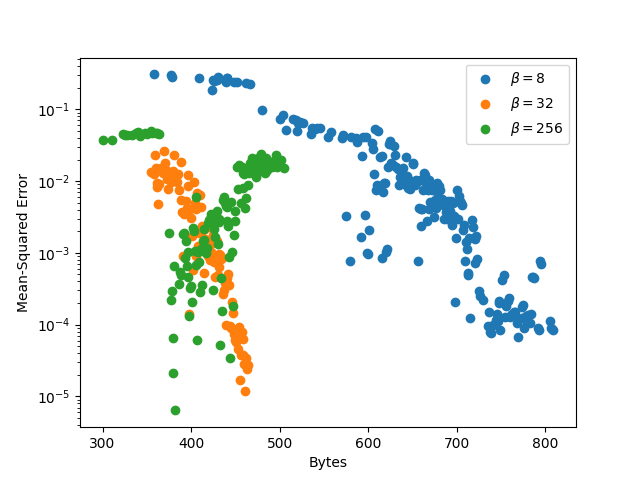
\includegraphics[width=\columnwidth]{diagrams/betas.png}
  \caption{Raster-encoding for several smoothing parameters. Increasing $\beta$ leads to better compression until reversing around $\beta=64$, when the surprisal becomes too expensive to allow switching colors often enough.}
  \label{fig:artifacts}
\end{figure}

Since a decoder would not have access to the original image, it can only compute probabilities using previously decoded pixels. Thus, we have to encode the pixels raster-wise, feeding back in the chosen value after each step. We choose values to minimize the following cost function:
$$\mathrm{cost}(x) = \mathrm{quality}\cdot(x-\mathrm{correct})^2-\log p(x).$$
A higher quality ensures the error is smaller, at the cost of using more bits. Since the decoder does not have access to future pixel values, we also mask the encoder's attention to only look at previous pixels. This has the added benefit of removing artifacts present with full attention (Figure \ref{fig:artifacts}).

\begin{figure}[h]
  \centering
  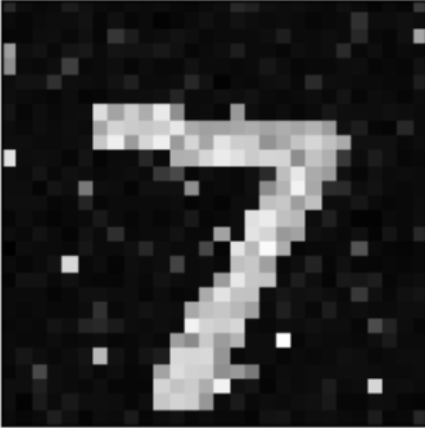
\includegraphics[width=0.25\columnwidth]{diagrams/artifacts.png}
  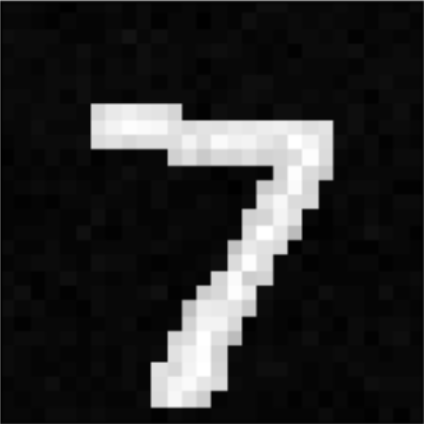
\includegraphics[width=0.25\columnwidth]{diagrams/no_artifacts.png}
  \caption{Full attention (left) vs. masked attention (right).}
  \label{fig:artifacts}
\end{figure}

\section{Results}
\begin{figure*}[h]
  \centering
  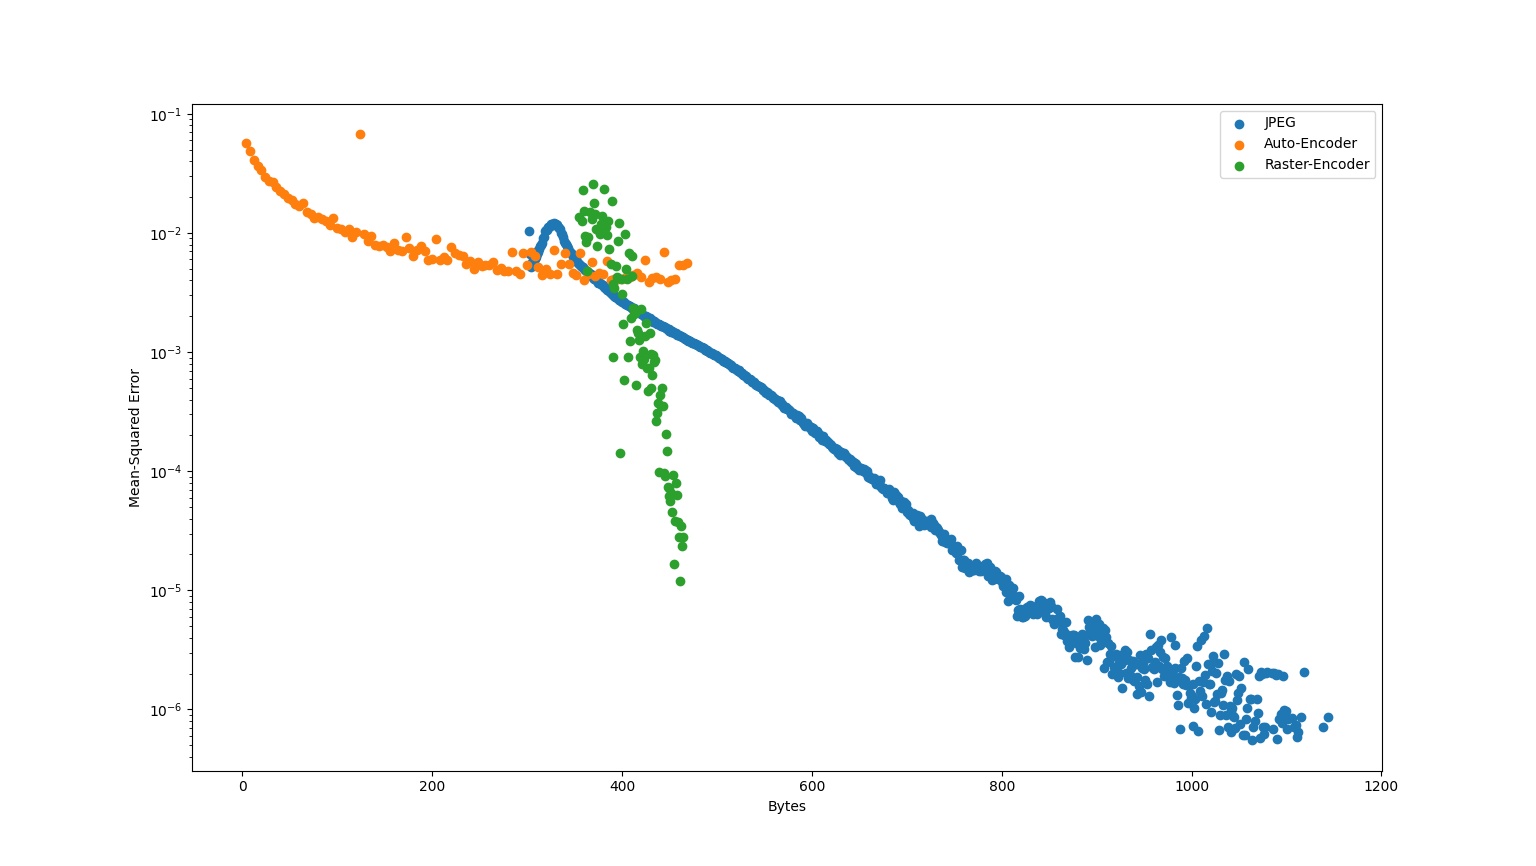
\includegraphics[width=2\columnwidth]{diagrams/results.png}
  \caption{Compression results.}
  \label{fig:results}
\end{figure*}

We find the auto-encoders outperform JPEG for small compression lengths, but flatten out at around $400$ bytes. This is likely because the convolutions only capture local features. Raster-encoders, which only capture global features, begin outperforming JPEG \emph{after} $400$ bytes (Figure \ref{fig:results}). A better compression scheme may combine the two, such as with vision transformers or LeCun's zip code recognition scheme \citep{lecun-1989-zip}.

\section{Further Discussion}


\bibliography{references}

\end{document}
